\documentclass[12pt, a4paper]{report} \usepackage[titletoc]{appendix}
%\linespread{1.5}
%\usepackage{lineno}
%\linenumbers
\usepackage{lscape}
\usepackage{enumitem}
\setlist[enumerate]{label*=\arabic*.}
\usepackage{makecell}
\usepackage{kantlipsum}
\usepackage{enumitem}
\usepackage{tabularx}
\usepackage{appendix}
\usepackage{multirow}
\usepackage{hhline}
\usepackage{array}
\usepackage{caption}
\usepackage{subcaption}
\usepackage{float}
\usepackage{graphicx}
\graphicspath{{images/}} 
\usepackage{geometry}
\geometry{a4paper,left=3cm,top=3cm,bottom=3cm,right=3cm}
\usepackage{array}
\usepackage{multirow}
\usepackage{hyperref}
\hypersetup{colorlinks=true,allcolors=blue}
\usepackage{hypcap}
\usepackage[linesnumbered,ruled]{algorithm2e}
\usepackage{courier}
\usepackage{listings}
\lstset{
basicstyle=\ttfamily,
frame=none, 
breaklines=true,
numbers=left,
xleftmargin=2.5em,
framexleftmargin=0em,
emphstyle=\textbf,
float=t
}
\lstdefinestyle{ocl}{
emph={
context, inv
}
}
\lstdefinestyle{change-based persistence}{
basicstyle=\ttfamily\scriptsize,
emph={
session, create, of, type,
set, to, add, hire
}
}
\lstdefinestyle{xmi}{
basicstyle=\ttfamily\scriptsize,
emph={
Node, children,
Employee, manages
}
}
\lstdefinestyle{xml}{
basicstyle=\ttfamily\scriptsize,
emph={
register, create, add, to, resource,
from, eattribute, remove, ereference,
set, unset, session, Roy, Jen,
Moss, Richmond
}
}
\lstdefinestyle{java}{
basicstyle=\ttfamily\scriptsize,
emph={
case, UNSET,
instanceof, else, if, void,
new, UnsetEAttributeEvent,
UnsetEReferenceEvent,
@override, public, class, extends
}
}
\lstdefinestyle{eol}{
basicstyle=\ttfamily\scriptsize,
emph={
var, new, for, in, create, set, of, with, 
unset, to, add, remove, delete, register,
from, position, from, move-within, session, \.
}
}

\setlength{\parindent}{1cm}
\setlength{\parskip}{0.1cm}


\begin{document}

\begin{titlepage}
\begin{center}

\textbf{Thesis Outline}
\vspace{1cm}

\textbf{\large Change-Based Model Persistence}
\vspace{1cm}

Alfa Ryano Yohannis\\
ary506@york.ac.uk
\vspace{1cm}

Supervisors:\\
Dimitris Kolovos\\
Fiona Polack\\
\vspace{1cm}

Department of Computer Science\\
University of York\\
United Kingdom\\
\vspace{1cm}
\today

\vfill

\end{center}
\end{titlepage}


\begin{abstract}
\addcontentsline{toc}{chapter}{Abstract}
Most of the models in Model-Driven Engineering are persisted in state-based formats. While state-based persistence has certain advantages, it is problematic when it comes to detecting changes in large-scale models. As an alternative, this work proposes a change-based approach that involves persisting the full sequence of changes made to models. Persisting models in a change-based format has the potential to deliver benefits over state-based persistence, such as the ability to detect changes much faster and more precisely, which can then yield positive knock-on effects on helping developers compare and merge models in collaborative modelling environments. Nevertheless, change-based persistence also comes with downsides, such as ever-growing model file sizes and increased model loading time. So far, an initial change-based persistence implementation for EMF models has been developed, and two approaches to optimise the loading of change-based models have been proposed: (1) an algorithm to ignore superseded events and (2) hybrid model persistence. Based on this work's interim results, the change-based approach persists changes in models faster than its state-based counterpart, the proposed algorithm loads change-based models faster than loading the models naively but it is still outperformed by loading models from state-based representation, and loading models from the hybrid model persistence only introduces a slight increase in loading and saving time. The initial implementation has been presented in a workshop paper, the proposed algorithm will be presented at a conference, and a paper discussing hybrid model persistence is currently under review. A research plan to complete this work in the next one and a half years is also presented in this report.
\end{abstract}

\tableofcontents
\addcontentsline{toc}{chapter}{Contents}

%\listoffigures
%\newpage

\listoftables
\newpage

%\lstlistoflistings
%\newpage

\chapter{Introduction}
\label{ch:introduction}
This Chapter briefly presents the background of this work as well as the research questions that will be addressed in this project. Several research objectives are then defined to answer the research questions. Lastly, research outputs and scoping are also presented. 

\section{Background}
\label{sec:background}
Most of the models in the context of Model-Driven Engineering are persisted in state-based formats. In such approaches, model files contain snapshots of the models' contents, and activities like version control and change detection are left to external systems such as file-based version-control systems and model differencing facilities. Activities such as change-detection (identifying parts that have changed in a model compared to a previous version) and model comparison (finding differences between models) are computationally consuming for state-based models \cite{Kolovos:2009:DMM:1564596.1564641}.  Thus, a new approach is needed to make the computation more efficient.

As an alternative to state-based persistence, this work proposes that a model can also be persisted in a change-based format, which persists the full sequence of \emph{changes} made to the model instead. The concept of change-based persistence is not new and has been used in persisting changes to software, object-oriented databases, and hierarchical documents \cite{DBLP:journals/entcs/RobbesL07,DBLP:conf/sde/LippeO92,DBLP:conf/caise/IgnatN05}. The change-based approach can improve detecting differences more precisely at the semantic level -- that is by providing finer-granularity information (e.g. types of changes, the order of the changes, elements that were changed, previous values, etc.) -- and therefore provide support to resolve them \cite{mens2002state}. The ordered nature of change-based persistence means that changes made to a model can be identified sequentially without having to explore and compare all elements of the model and its previous version. Based on these arguments, this work explores the advantages and shortcomings of change-based persistence as an alternative approach to state-based persistence for models conforming to 3-layer metamodelling architectures such as EMF and MOF. Persisting models in a change-based format can bring a number of envisioned benefits over state-based persistence, such as the ability to detect changes much faster and more precisely, which can then have positive knock-on effects on supporting (1) developers compare and merge models in collaborative modelling environments, and (2) incremental model management ( e.g. incremental query \cite{DBLP:conf/ecmdafa/RathHV12} and model-to-text transformation \cite{Ogunyomi2018}). 

Nevertheless, change-based persistence also comes with downsides, such as ever-growing model files \cite{DBLP:journals/entcs/RobbesL07,DBLP:conf/edoc/KoegelHLHD10} and increased model loading time \cite{mens2002state} which increase storage and computation costs. A model that is frequently modified will increase considerably in file size since every change is added to the file. The increased file size (proportional to the number of persisted changes) will, in turn, increase the loading time of the model since all changes have to be replayed to reconstruct the model's eventual state. These downsides have to be mitigated to enable the practical adoption of change-based persistence. One approach to reducing the file size of change-based models is by removing changes that do not affect the eventual state of the model. For the increased loading time, it can be mitigated by ignoring -- i.e. not replaying -- changes that are cancelled out by later changes or employing change-based and state-based persistence side-by-side so that the benefits of state-based persistence on loading time can be obtained. Other downsides are change-based persistence requires integration with existing tools -- since it is still a non-standard approach -- for its adoption \cite{koegel2010emfstore}, and still has limited support for standard, text-based version controls for collaborative development \cite{koegel2010emfstore}. These downsides can be addressed by developing a change-based persistence plugin for a specific development environment (e.g. Eclipse) and persisting changes in text-based format to support text-based version controls (e.g. Git, SVN).

\section{Research Questions}
\label{sec:research_questions}
The hypothesis of this work is that \textbf{``Change-based persistence reduces the execution time of model change-detection, model comparison, and model merging for large models compared to their execution time in state-based persistence, with acceptable trade-offs on loading and persisting time, memory footprint, and storage space consumption''}. The execution time is the time required to complete the processes (e.g. change-detection, model comparison, model merging, or persisting changes). Model change-detection is identifying changed elements of a model compared to its previous version/ancestor while the model comparison is finding the differences between two models that come from the same ancestor. Model merging is reconciling two models that come from the same ancestor and combining them to produce a new model. Using the term ``large models'' we refer to models with more than 1M elements, consistently with \cite{daniel2016neoemf,DBLP:conf/models/Espinazo-PaganCM11}. Model load time is the amount of time required to load a model into memory. Persisting changes is saving changes made to a model into a persistent representation (e.g. a file). Memory footprints are the sizes of memory used to execute the processes. Disk space consumption is the amount of storage consumed by the persistence.

To assess the validity of the hypothesis, this work aims to answer the following research questions: 
\begin{enumerate} 
\item \textbf{How to persist models in a change-based format? How does it perform compared to state-based persistence on saving changes?} 

The concept of change-based persistence has to be translated into an implementation in a modelling framework context so that it can be applied for model persistence, and therefore its impact on model change-detection, model comparison, and model merging can be assessed.
%It is expected that every change made to a model can be persisted by the implementation. Replaying all the persisted changes can reconstruct the same model as the model persisted in state-based format. 
%It is also expected that change-based persistence will outperform state-based persistence on time required for saving changes since change-based persistence will only require persisting changes of a model while state-based persistence will persist the whole model. 

%\item \textbf{How to mitigate the ever-growing file size and increased loading time of change-based models? To what extent can they be reduced?} 
%
%Change-based persistence comes with the downsides of larger file sizes and increased loading time. Mitigating these side effects will is essential for facilitating the practical adoption of change-based persistence. For the increased file size, the size can be reduced by removing changes that do not affect the eventual state of the model. For the increased loading time, it can be mitigated by ignoring -- not replaying -- changes that are cancelled out by subsequent changes or employing change-based and state-based persistence side-by-side (hybrid approach). Employing both persistence side-by-side can maintain the benefit of state-based persistence on loading time. It is expected that the mitigation approaches will (1) lead to loading time that is closer to the loading time of state-based format, (2) significantly load models faster than loading change-based models naively, and (3) significantly reduce change-based model file sizes compared to the naive approach on saving change-based model files. 
%
%For reducing the loading time using change-based and state-based persistence side-by-side, the impact of the approach will also be investigated on several qualities. It is expected that a hybrid persistence approach will: (1) be significantly slower than change-based persistence on persisting changes and slightly slower than state-based persistence on saving time as the hybrid approach will need to save changes to the other two types of persistence, (2) consume more disk space compared to change-based or state-based persistence since the hybrid approach will use them both simultaneously, and (3) facilitate loading time that is closer to the loading time of state-based persistence. 

\item \textbf{How to detect changes in change-based models -- comparing them to their ancestors/previous versions? To what extent does change-detection in change-based models perform compared to change-detection in state-based models?} 

The purpose of using change-based persistence in this work is to improve change-detection. The change-based persistence will have change-detection time that is smaller than the change-detection time of state-based persistence.        

\item \textbf{How to compare change-based models that come from the same ancestor? How does the comparison of change-based models perform compared to the state-based model comparison?} 

The knock-on effect of faster change-detection on model comparison will also be investigated. Due to the nature of change-based models, the mechanism to perform change-based model comparison will differ substantially from the current state-based model comparison. It is expected that comparison of change-based models will be significantly faster than the comparison of state-based models.

\item \textbf{How to merge different change-based models that come from the same ancestor? How does the merging perform compared to model merging in state-based persistence?}

Another knock-on effect of faster change-detection of change-based persistence is faster model merging. Similar to the change-based model comparison, the mechanism to merge change-based models will differ substantially from merging state-based models. It is expected that the change-based model merging will be much faster than state-based model merging.   

\end{enumerate}

\section{Research Objectives}
\label{sec:research_objectives}
This research aims to meet the following research objectives to answer the research questions.
\begin{enumerate}
\item Develop an implementation of change-based persistence so it can be applied to persist models in change-based format, and evaluate the correctness of change-based models that it produces and its performance on saving changes against state-based persistence. 
\item Develop a solution to detect changes in change-based models, and compare its execution time and memory footprint against change-detection in state-based models.
\item Develop a solution to compare change-based models, and compare its execution time and memory footprint against model comparison in state-based models.
\item Develop a solution to merge different change-based models, and compare its execution time and memory footprint against model-merging in state-based models. 
\end{enumerate}

\section{Research Outputs}
\label{sec:research_outputs}
By the end of this research, these following outputs will have been produced:
\begin{enumerate}
\item Prototypes for change-based persistence. 
\item Solutions -- including their implementation and evaluation -- for file size and loading time reduction, change-detection (finding parts that already changed of a model compared to its previous version/ancestor), model comparison (finding differences between models that come from the same ancestor), and model merging of change-based persistence.
\item Publications and a thesis documenting the outcomes of this research.
\end{enumerate}


\section{Research Scope}
\label{sec:research_scope}
The scope of this research will be restricted to models conforming to 3-level metamodelling architectures. The Eclipse Modelling Framework will be used, as a representative example of such architectures, for the implementation of all algorithms and prototypes.

%All prototypes in this research will be developed on top of Eclipse Modelling Framework. Since this research will also use change-based and state-based persistence side-by-side, an existing instance of state-based persistence is required for executing the implementation and evaluation. NeoEMF \cite{daniel2016neoemf}, a recent work that leverages the use of NoSQL databases for large-scale model persistence, is considered pertinent for this research. Also, the change-based persistence only records changes made to a model. Changes made to a model's metamodel are outside the scope of this research. Moremover, persisted changes are immutable. It means that they cannot be altered to preserve the entire history of a model.

\chapter{Thesis Structure}
\label{sec:Thesis Structure}
This section provides the description of the planned thesis structure. Each subsection corresponds to a chapter in the thesis report and describes the purpose and contents of the chapter. Some of the contents have been discussed in this research's Progress Report \cite{yohannis2017progress} and written papers \cite{DBLP:conf/models/YohannisKP17,yohannis2018towards,yohannis2018hybrid}, and they will be transferred to the thesis report with proper adjustments. The time frame for each chapter is presented in Chapter \ref{ch:plan}.

\section{Chapter 1: Introduction}
\label{sec:chapter_1_introduction_plan}
This chapter will present the motivation and purpose of this research. It will comprise the (1) background of the research as well as the (2) research hypothesis, (3) research questions, (4) research objectives, (5) research outputs, and (6) research scope. All of these contents have been defined in the Progress Report \cite{yohannis2017progress} and  this Thesis Outline, and they will be transferred to the Thesis Report with proper adjustments. 


\section{Chapter 2: Literature Review}
\label{sec:chapter_2_literature_review_plan}
This chapter will summarise work related to change-based persistence and comparison, critically assesses the advantages and disadvantages of current approaches, and seek the opportunities to contribute novel knowledge to the field. The chapter will comprise (1) change-based approaches in software engineering, (2) change-based model persistence, (3) state-based model persistence, (4) text-based comparison and merging, (5) state-based model comparison and merging, and (6) change-based model comparison and merging. Most of these topics have been discussed briefly in the Progress Report \cite{yohannis2017progress}. However, text-based comparison, state-based model comparison, and change-based model comparison and merging need more literature review and deeper analysis to support defining a new approach for change-based model comparison and merging.


\section{Chapter 3: Change-based Model Persistence}
\label{sec:chapter_3_Change-based_model_ersistence_plan}
This chapter will present the concept of change-based model persistence and its core implementation. The chapter will comprise the concept of change-based model persistence, and the design of the core implementation. The implementation is evaluated by comparing the eventual model produced by replaying a change-based representation to the same model but loaded from a state-based persistence (e.g. XMI). These contents have been published in a workshop \cite{DBLP:conf/models/YohannisKP17}.


\section{Chapter 4: Optimised Loading of Change-based Model Persistence}
\label{sec:chapter_4_optimised_loading_change_based_model_persistence}

Change-based persistence comes with a downside of ever-growing file sizes \cite{DBLP:journals/entcs/RobbesL07,DBLP:conf/edoc/KoegelHLHD10} which causes increased loading time \cite{mens2002state}. Reducing the loading time is essential to facilitate the practical adoption of change-based persistence. One way to reduce the increased loading time is by ignoring -- not replaying -- changes that are cancelled out by subsequent changes. 

To evaluate the efficiency of the proposed approach, the optimised loading is compared to a naive loading of a change-based representation and loading the same model from a state-based representation. They are compared on time required to load models and the memory footprint after loading models. Evaluation is also performed on time required for persisting changes between change-based and state-based persistence to show the benefit of change-based persistence on saving changes. 

This chapter will present the optimisation approach along with its implementation and evaluation. The contents of this chapter will be largely based on an accepted conference paper \cite{yohannis2018towards}. 


\section{Chapter 5: Hybrid Model Persistence}
\label{sec:chapter_5_hybrid_model_persistence}
While optimised loading is faster than the naive loading, the benefits are moderate and that the optimised loading is still slower than loading from a state-based representation \cite{yohannis2018towards}. This finding has motivated the design and development of a hybrid persistence approach, that is augmenting a change-based representation with a state-based representation. 

The hybrid model persistence approach is evaluated by comparing it to state-based persistence (e.g. XMI, NeoEMF \cite{daniel2016neoemf}) on time, memory footprint, and storage space required for loading models and persisting changes. The evaluation is also performed on time required for detecting changes between hybrid and state-based persistence to show the benefit of change-based persistence over state-based model comparison. 

This chapter will present the hybrid model persistence approach together with its implementation and evaluation. The contents of this chapter will be largely based on a conference paper \cite{yohannis2018hybrid} that is currently under review. 

\section{Chapter 6: Change-based Model Comparison}
\label{sec:chapter_6_change_based_model_comparison}
This chapter will present a change-based model comparison algorithm with its implementation and evaluation. Change-based persistence is expected to speed-up model comparison because the information required to identify changes is already contained in the models' representation. 

The proposed algorithm will be evaluated by comparing it to state-based model comparison (e.g. EMF Compare \cite{eclipse2017compare}) on the time and memory footprint required to find all differences between models. This research will derive synthetic models from branches of real-world software projects as datasets in the evaluation. The alternative strategy is to perform an experiment on modellers. They will be asked to develop models in parallel. The produced models will be upscaled and used in the evaluation. 

The findings of this chapter will be published together with the findings of Chapter 7.


\section{Chapter 7: Change-based Model Merging}
\label{sec:chapter_7_change_based_model_Merging}
This chapter will present change-based model merging. After identifying the differences between two versions of a change-based model, there is a need to reconcile all the differences into a new version of the model. Thus, conflicts between the two versions have to be identified and resolved -- using predefined rules or based on users' decisions, and by then merging steps can be determined to merge the two versions. 

Similar to change-based model comparison in Section \ref{sec:chapter_6_change_based_model_comparison}, the proposed merging approach will also be evaluated by comparing it to the merging of state-based persistence (e.g. EMF Compare) on the affected time and memory footprint. The evaluation will also use the same datasets in Section \ref{sec:chapter_6_change_based_model_comparison}.

The findings of this chapter will be published together with the findings of Chapter 6.

\section{Chapter 8: Conclusions and Future Work}
\label{sec:chapter_8_conclusions}
This chapter will present the conclusions of this research as well as the future work. 

%\begin{enumerate}
%    \setlength\itemsep{0pt}
%\item Conclusions from every chapter.
%\item Future work.
%\end{enumerate}

\chapter{Plan}
\label{ch:plan}
This Chapter presents the outstanding tasks for each chapter in the thesis report and the estimated time to complete the tasks. The timetable for the remaining tasks of this research can be seen in Table \ref{table:timetable}.

\begin{enumerate}
    \setlength\itemsep{0pt}
    \item \textbf{Chapter 1: Introduction}
    \begin{enumerate}
        \item \textit{Writing Up}
        \begin{enumerate}
            \item Transfer this chapter to the thesis report. (estimated time: 5 days)
        \end{enumerate}
    \end{enumerate}
    \item \textbf{Chapter 2: Literature Review}
    \begin{enumerate}
        \item \textit{Review Work}
        \begin{enumerate}
            \item Review related work on the text-based comparison and merging, state-based model comparison and merging, and change-based model  comparison and merging. (10 days)
        \end{enumerate}
        \item \textit{Writing Up}
        \begin{enumerate}
            \item Transfer the literature review to the thesis report. (5 days)
        \end{enumerate}
    \end{enumerate}
    \item \textbf{Chapter 3: Change-based Model Persistence}
    \begin{enumerate}
        \item \textit{Writing Up}
        \begin{enumerate}
            \item Transfer the related written paper to the thesis report. (5 days)
        \end{enumerate}
    \end{enumerate}
    \item \textbf{Chapter 4: Optimised Loading of Change-based Model Persistence}
    \begin{enumerate}
        \item \textit{Writing Up}
        \begin{enumerate}
            \item Transfer the related written paper to the thesis report. (5 days)
        \end{enumerate}
    \end{enumerate}
    \item \textbf{Chapter 5: Hybrid Model Persistence}
    \begin{enumerate}
        \item \textit{Writing Up}
        \begin{enumerate}
            \item Transfer the related paper to the thesis report. (5 days)
        \end{enumerate}
    \end{enumerate}
    \item \textbf{Chapter 6: Change-based Model Comparison}
    \begin{enumerate}
        \item \textit{Research}
        \begin{enumerate}
            \item Develop a solution for change-based model comparison. (15 days)
            \item Develop an implementation of the solution. (15 days)
            \item Evaluate the solution. (10 days)
        \end{enumerate}
    \end{enumerate}
    \item \textbf{Chapter 7: Change-based Model Merging}
    \begin{enumerate}
        \item \textit{Research}
        \begin{enumerate}
            \item Develop a solution for change-based model merging. (15 days)
            \item Develop an implementation of the solution. (15 days)
            \item Evaluate the solution. (10 days)
        \end{enumerate}
        \item \textit{Publication}
        \begin{enumerate}
            \item Write a paper for chapters 6 and 7. (20 days)
        \end{enumerate}
        \item \textit{Writing Up}
        \begin{enumerate}
            \item Transfer the related paper to the thesis report. (5 days)
        \end{enumerate}
    \end{enumerate}
    \item \textbf{Chapter 8: Conclusions and Future Work}
    \begin{enumerate}
        \item \textit{Writing Up}
        \begin{enumerate}
            \item Write conclusions and future works. (5 days)
        \end{enumerate}
    \end{enumerate}
\end{enumerate}

\begin{landscape}

\begin{table}[h]
\centering
\caption{The time table for the remaining tasks of this research. One week consists of 5 working days. }
\label{table:timetable}
\centering
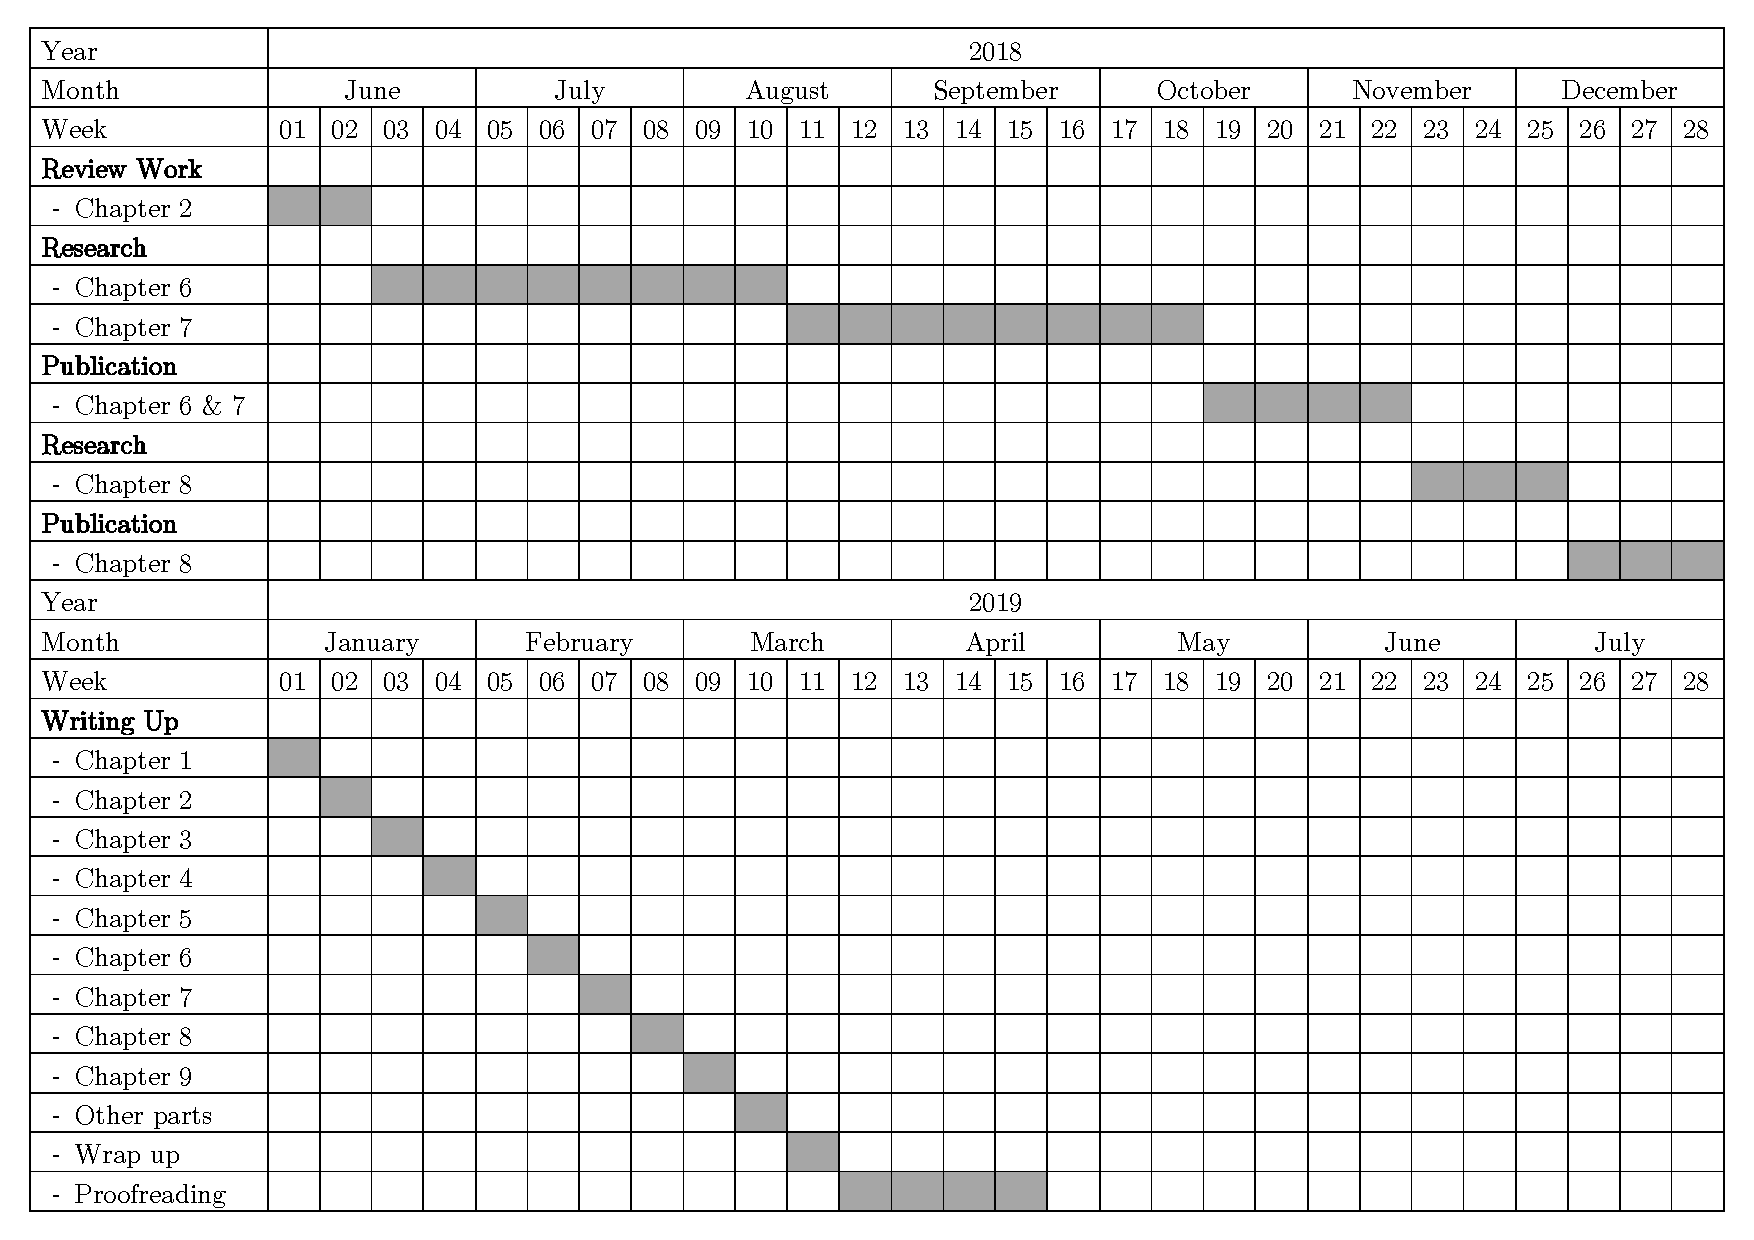
\includegraphics[width=0.95\linewidth]{images/timetable}
\label{fig:timetable}
\end{table}
\end{landscape}



\chapter{Publications}
\label{ch:publications}
Three papers have been written. The first paper \cite{DBLP:conf/models/YohannisKP17} has been presented in the FlexMDE 2017 workshop, the second paper \cite{yohannis2018towards} has been accepted and will be presented at the ECMFA 2018 conference, and the third paper \cite{yohannis2018hybrid} has been submitted to ASE 2018 and is currently under review. These papers can be found in Appendices.
\begin{enumerate}
\item A. Yohannis, F. Polack, and D. Kolovos, ``Turning Models Inside Out," in Proceedings of the 3rd Workshop on Flexible Model Driven Engineering co-located with ACM IEEE 20th International Conference on Model Driven Engineering Languages and Systems (MoDELS 2017), 2017.
\item  A. Yohannis, H. Hoyos Rodriguez, F. Polack, and D. Kolovos, ``Towards Efficient Loading of Change-based Models," in Proceedings of the 14th European Conference on Modelling Foundations and Applications (ECMFA 2018) co-located with Software Technologies: Applications and Foundations (STAF 2018), 2018 (to be presented).
\item  A. Yohannis, H. Hoyos Rodriguez, F. Polack, and D. Kolovos, ``Towards Hybrid Model Persistence," submitted to the 33rd IEEE/ACM International Conference on Automated Software Engineering (ASE 2018), 2018 (under review).
\end{enumerate}


\bibliographystyle{IEEEtran}
\bibliography{references}

%\begin{appendices}
%\end{appendices}

\end{document}